\documentclass[12pt]{article}

\title{\vspace*{55mm}\Huge\textbf{Software Systems Lab: Outlab 5} \\ \textbf{\LaTeX (80 marks)}}
\author{\huge Dominatrix \\ \\ \large 180050005 \\ 180050095 \\ 18D070026}
\date{14 September, 2019}

\usepackage{geometry}
\usepackage{amsmath}
\usepackage{amssymb}
\usepackage{hyperref}
\usepackage{ulem}
\usepackage[T1]{fontenc}
\usepackage[utf8]{inputenc}
\usepackage{imakeidx}
\usepackage{sectsty}
\usepackage{titling}
\usepackage{graphicx}
\usepackage[shortlabels]{enumitem}
\geometry{a4paper,total={6in,9in},left=3cm,top=1in}
\sectionfont{\fontsize{17}{5}\selectfont}
\setlength{\parindent}{0.7 em}
\newcommand{\LATEX}{\LaTeX}
\newcommand{\comment}[1]{}
\usepackage{bera}
\usepackage{multirow}
\usepackage{caption}
\usepackage{subcaption}

\graphicspath{{./}}
\begin{document}

\fontdimen2\font=0.4ex

\begin{titlingpage}
	\maketitle
\end{titlingpage}
\newpage
\tableofcontents


\newpage

 This is a \LaTeX document for the course \textbf{Software Systems Lab} with course code \textit{CS 251}. You need to replicate the document. Spacing need not be matched perfectly but page numbers should be. \textbf{1 mark is for the title page}. Bonus marks will be given only if you score full (80/80) in the rest.

 
\section{ Introduction (4 marks) }%fontsize of introduction to be reduced
\indent

\textbf{\LaTeX} is a word processor and document markup language. It is distinguished from typical word processors such as Microsoft Word and Apple Pages in that the writer uses plain text as opposed to formatted text, relying on markup tagging conventions to define the general structure of a document (such as article, book, and letter), to stylise text throughout a document (such as \textbf{bold} and italic), and to add citations and cross-referencing. A \textbf{\TeX} distribution such as \textbf{\TeX} \textbf{Live} or \textbf{MikTeX} is used to produce an output file (such as PDF or DVI)
suitable for printing or digital distribution.
\newline

 
\textbf{\LaTeX} is used for the communication and publication of scientific documents
in many fields, including mathematics, physics, computer science, statistics,
economics, and political science. It also has a prominent role in the preparation
and publication of books and articles that contain complex multilingual materials, such as Sanskrit and Arabic. \textbf{\LATEX} uses the TeX typesetting program for
formatting its output, and is itself written in the TeX macro language.
\newline


\textbf{\LaTeX} is widely used in academia. \textbf{\LaTeX} can be used as a standalone document preparation system, or as an intermediate format. In the latter role, for
example, it is often used as part of a pipeline for translating DocBook and other
XML-based formats to PDF. The typesetting system offers programmable desktop publishing features and extensive facilities for automating most aspects of
typesetting and desktop publishing, including numbering and cross-referencing
of tables and figures, chapter and section headings, the inclusion of graphics,
page layout, indexing and bibliographies.\newline
\par


Below are some of the basic packages which you’ll be using. For other
required packages, search over the net :).
\par


\subsection {graphicx package}
This package is used to import tables, and figure in the document. Our
document type is article, and we are currently using a4 type paper with the
following margin geometry: (total={6in, 8in}, margin=1.2in, bottom=1in),
which is specified in the beginning.

\subsection {amssymb package}
This package is used to import mathematical symbols in the document. We
encapsulate the mathematical equations and symbols under \$, and they are
changed to maths symbols.
 
\section{Pointers (3 + 2 + 1 marks)}
Here we are using \textbf{itemize} to generate unordered list.
%\renewcommand\labelitemi{\large$\bullet$} %baad me karenge
\begin{itemize}
 
 \setlength\itemsep{1em}
	\item \LATEX typesets a file of text using the TEX program.
	\item \LATEX is widely used in academia for the communication and publication of scientific documents in many fields, including mathematics, physics, computer science, statistics, economics and political science.
	\item \LATEX can be used as a standalone document preparation system or as an intermediate format.
	\item \textbf{We have used renewcommand for the bullets to be bigger.}
	\item Look at the \textbf{item separation space}, and \textbf{change it} accordingly.
\end{itemize}

For ordered lists we use enumerate.

\begin{enumerate}[label=\Roman*]
\item \LATEX typesets a file of text using the TEX program.
\item \LATEX is widely used in academia for the communication and publication
of scientific documents in many fields, including mathematics, physics,
computer science, statistics, economics and political science.
\item \LaTeX can be used as a standalone document preparation system or as an
intermediate format.
\item \LATEX is intended to provide a high-level language that accesses the power
of TeX in an easier way for writers.

\end{enumerate}

\begin{enumerate}[(a)]
\item \LATEX typesets a file of text using the TEX program.
\item \LATEX is widely used in academia for the communication and publication
of scientific documents in many fields, including mathematics, physics,
computer science, statistics, economics and political science.
\end{enumerate}

Following is another type of a pointer (\textbf{description}).


\textbf{CS 213} Data Structures and Algorithm
%need to have some spaces between lines
\textbf{CS 215} Data analysis and interpretation
\newpage

\section{Mathematical formulae and notations (15 marks)}

\subsection{Equation Array (4 marks)}

\begin{eqnarray} \label{eq1}
cos^3\theta + sin^3\theta & = & (cos\theta + sin\theta)(cos2\theta - cos\theta sin\theta) \\
& = & (cos\theta + sin\theta)(1 - cos\theta sin\theta) \\
& = & (cos\theta + sin\theta)(1/2)(2 - 2cos\theta sin\theta)(3) \\
& = & (1/3)(cos\theta + sin\theta)(2-sin2\theta)
\end{eqnarray}

\subsection{Prepositional Formulae using Various Operators (2 marks)}
\begin{eqnarray*}
(\exists x) (\phi(x)\wedge\psi(x)) & \longleftrightarrow & ((\exists x) \phi(x) \wedge (\exists x) \psi(x)) \\
(\exists x)  (\phi(x) \wedge \psi(x)) & \longrightarrow & ((\exists x) \phi(x) \wedge (\exists x) \phi(x) \wedge (\exists x) \psi(x))
\end{eqnarray*}
%not appropriate spaces between equation expressions neither left aligned

\comment{
\begin{eqnarray*}
$cos^3θ + sin3
θ = (cosθ + sinθ)(cos2θ − cosθsinθ) (1)
= (cosθ + sinθ)(1 − cosθsinθ) (2)
= (cosθ + sinθ)(1/2)(2 − 2cosθsinθ)(3) (3)
= (1/2)(cosθ + sinθ)(2 − sin(2θ)) (4)$
}
Figure 2: Screenshot: Generated Notification


\subsection{Alphabets (3 marks + 1 mark for table)}
\medskip
\begin{center}

\begin{tabular}{ |c|c| }
\hline
Binary Operators: & $\times$   $\otimes$   $\oplus$   $\cup$   $\cap$  \\ [3 ex]
\hline
Relation Operators: & $\subset$   $\supset$    $\subseteq$    $\supseteq$    $< >$ \\ [3 ex]
\hline
Others : & $\int$   $\oint$    $\Sigma$    $\Pi$ \\ [3 ex]
\hline
\end{tabular}
\end{center}





\newpage



\section{Tables (10 marks)}
\indent
To combine rows a package must be imported with in your preamble, then you
can use the XXXXXXX command in your document. The table below includes
mathematical notations, which you can produce by embedding the expression
in $ $ delimiters. For subscript, use underscore and for superscript, use carrot. \\ \\
\newpage

\section{Image Insert (7 + 7 marks)}

\hspace{1.5 ex} \hspace{2 ex} Now, we will import images side by side in the same document.
\begin{figure}[!h]
\begin{subfigure}[t]{.37\textwidth}
  \centering
  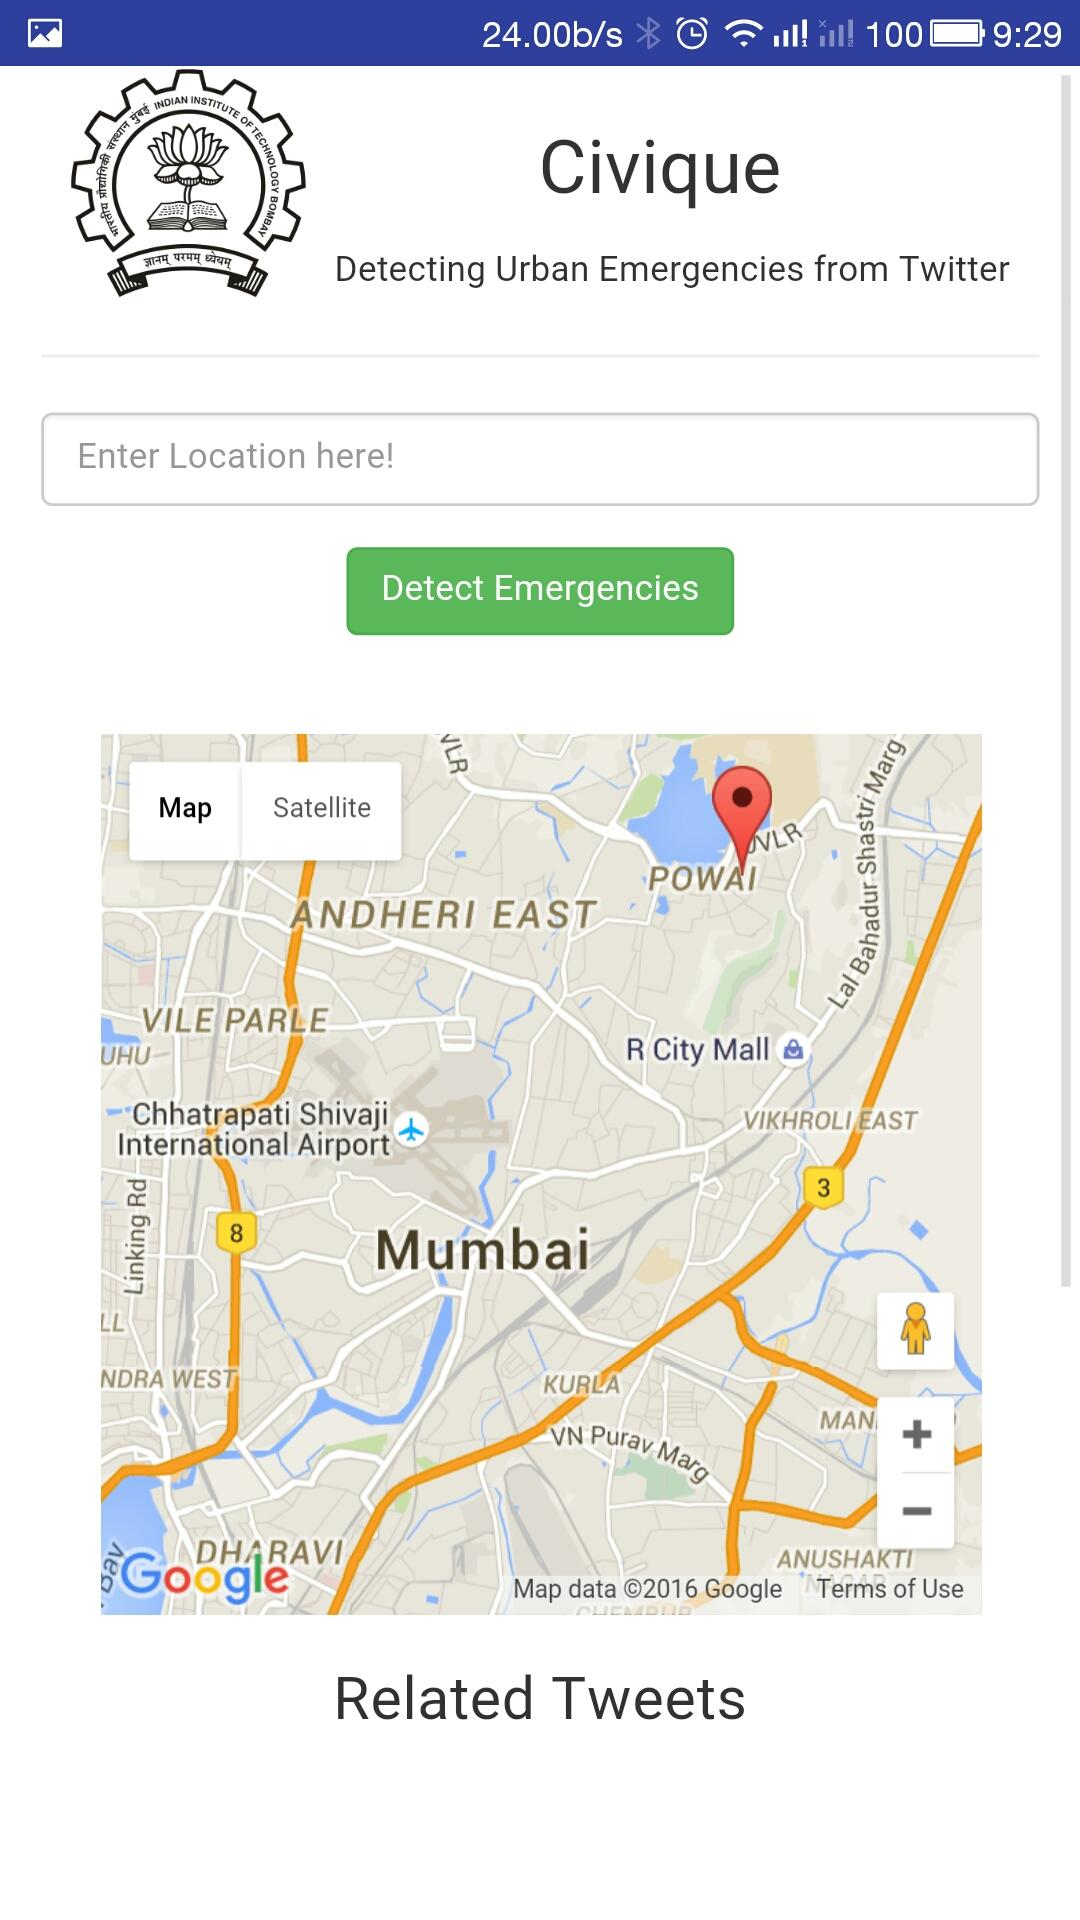
\includegraphics[width=.65\linewidth]{1}
  \caption*{Figure 1: Screenshot: Mobile
Interface}
  \label{fig:sub1}
\end{subfigure}%
\begin{subfigure}[t]{.37\textwidth}
  \centering
  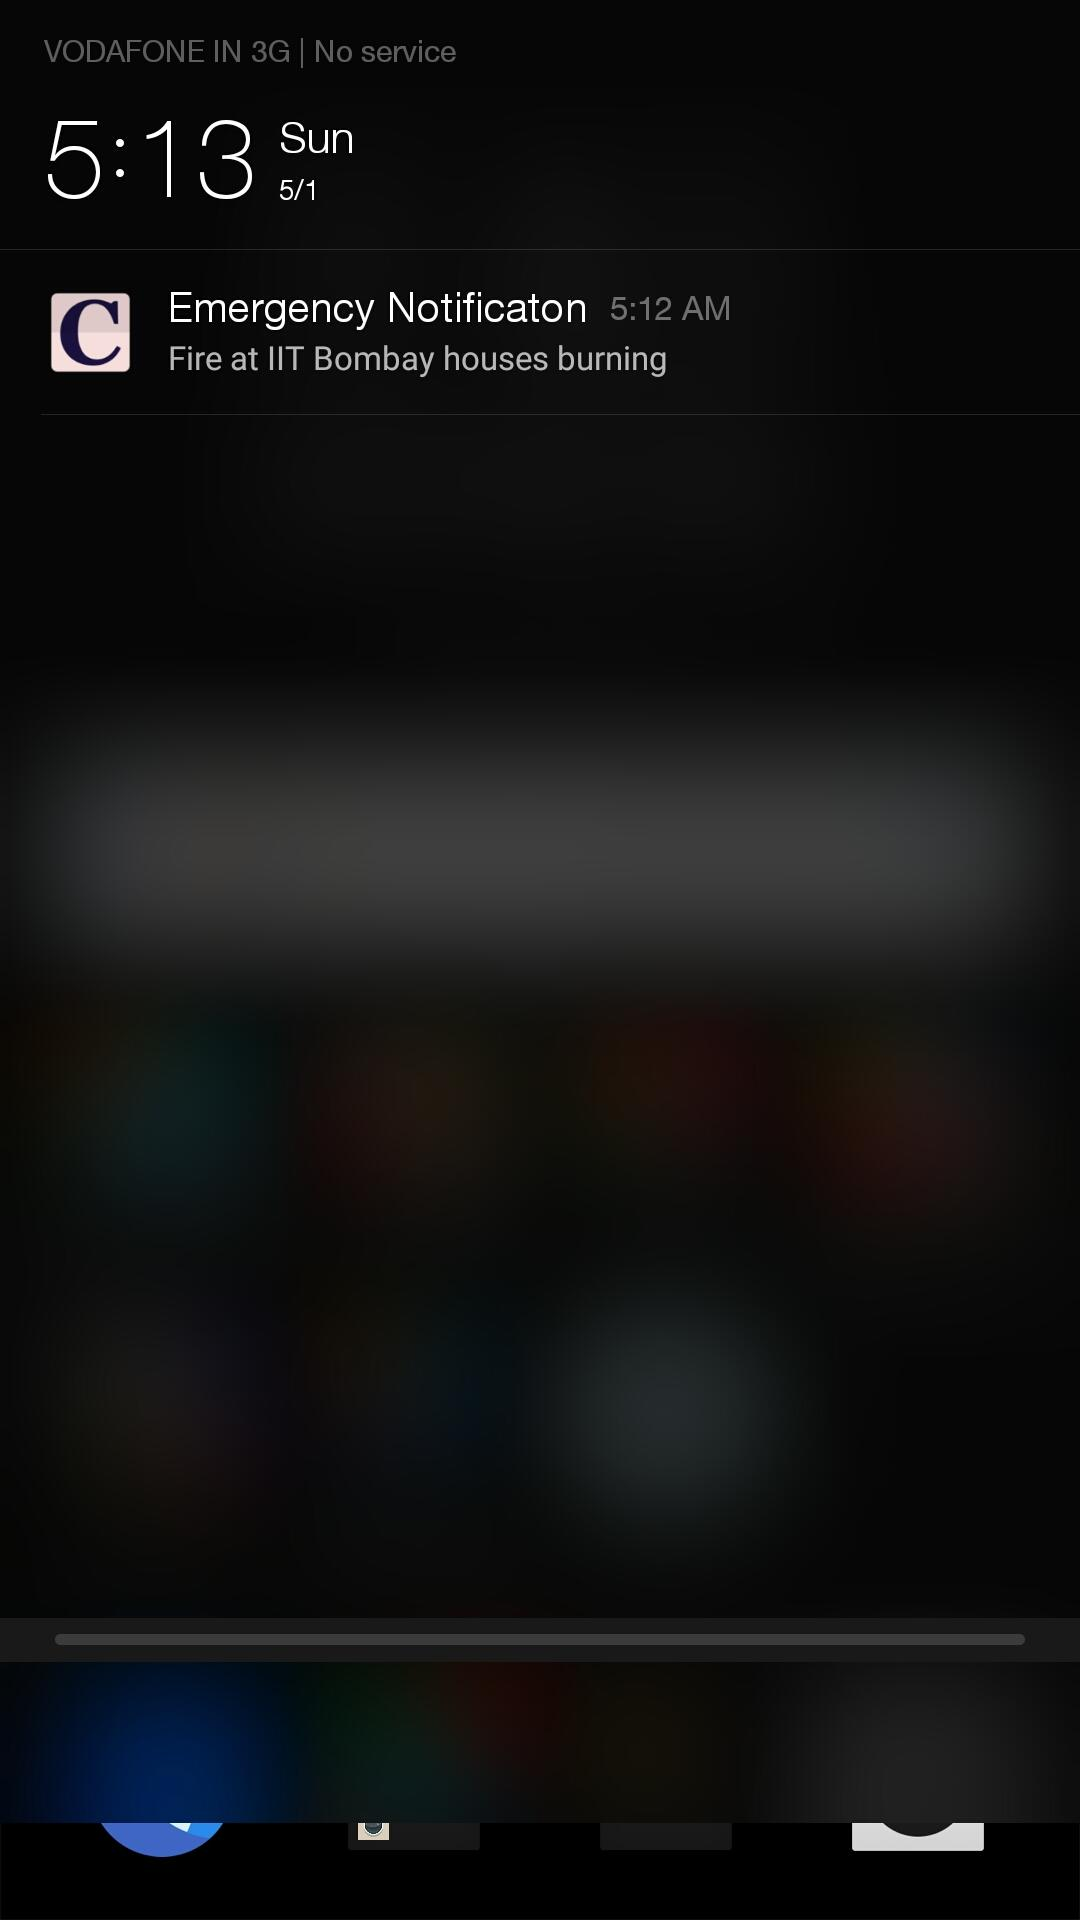
\includegraphics[width=.65\linewidth]{2}
  \caption*{Figure 2: Screenshot: Generated Notification}
  \label{fig:sub2}
\end{subfigure}
\end{figure}
\end{document}
